\chapter{Mutant npat results in nucleosome positioning defects in \textit{D. rerio} CMZ progenitors, preventing specification but not proliferation}
\label{chap:rys}
\section{Introduction}
The zebrafish (D. rerio) circumferential marginal zone (CMZ), located in the retinal periphery, contains the retinal stem cells and progenitors responsible for the lifelong retinal neurogenesis observed in this cyprinid. Analagous to CMZs in other model organisms, such as X. laevis \cite{Perron1998}, it has been of particular interest to us since the discovery of quiescent stem cells at the mammalian retinal periphery \cite{Tropepe2000}, as an understanding of the molecular mechanisms regulating this proliferative zone may shed light on whether these mammalian cells might be harnessed for the purpose of regenerative retinal medicine. While significant progress has been made in this direction \cite{Raymond2006}, molecular lesions in a plethora of zebrafish mutants displaying defects in CMZ development and activity remain largely uncharacterised. We examine here one such micropthalmic line identified in an ENU screen, rys \cite{Wehman2005}, characterised by Wehman et al. as a Class IIA CMZ mutant, with an apparently paradoxically enlarged CMZ.

Mapping revealed the causative rys mutation lay in the zebrafish npat gene, the nuclear protein associated with the ataxia-telangiectasia locus in mammals \cite{Imai1996}. Although npat is heretofore uncharacterised in zebrafish, its mammalian homologues, human NPAT and mouse Npat, have been extensively examined. These studies have demonstrated that NPAT plays a critical role in coordinating events associated with the G1/S phase transition in proliferating cells \cite{Ye2003}. S-phase entry requires tight co-ordination between the onset of genomic DNA synthesis and histone production, in order to achieve normal chromatin packaging and assembly. NPAT, found in the nucleus \cite{Sagara2002} and localised, in a cell-cycle dependent manner, to histone locus bodies \cite{Ghule2009}, induces S-phase entry \cite{Zhao1998} and activates replication-dependent histone gene transcription by direct interaction with histone gene clusters \cite{Zhao2000} in association with histone nuclear factor P (HiNF-P) \cite{Mitra2003}. The protein’s effects on S-phase entry and histone transcription are associated with distinct domains at the C-terminus and N-terminus, respectively \cite{Wei2003}. NPAT is also known to associate with the histone acetyltransferase CBP/p300 \cite{Wang2004} and directs histone acetylation by this enzyme \cite{He2011}.

NPAT is known to be a component of the E2F transcriptional program \cite{Gao2003} and a substrate of cyclin E/CDK2 \cite{Zhao1998}, although E2F-independent activation by cyclin D2/CDK4 in human ES cells has also been described \cite{Becker2010}. The expression of NPAT protein peaks at the G1/S boundary \cite{Zhao1998}, as does its phosphorylation, which promotes its transcriptional activation of replication-dependent H2B \cite{Ma2000} and H4 \cite{Mitra2009} genes, while its effect on low, basal levels of H4 transcription is phosphorylation-independent \cite{Ye2003}. Of particular interest, NPAT has recently been found to be required for CDK9 recruitment to replication-dependent histone genes (Pirngruber and Johnsen, 2010); CDK9 and monoubiquitinated H2B are essential for proper 3’ end processing of stem-loop histone transcripts \cite{Pirngruber2009}. NPAT and HiNF-P have also been found associated with the U7 snRNP complexes that perform this function \cite{Ghule2009}. The replication-dependent activities of NPAT are thought to be terminated by WEE1 phosphorylation of H2B, which excludes NPAT from histone clusters \cite{Mahajan2012}.

All of these studies have been conducted in tissue culture contexts, perhaps due to the challenges associated with studying this critical protein in vivo; mouse embryos with provirally inactivated Npat arrest at the 8-cell stage, for instance \cite{DiFruscio1997}. The availability of rys, a zebrafish npat mutant which develops well into the larval stage, is therefore of considerable interest, as it allows for the study of npat’s function within complete tissues. We demonstrate here that npat is critical for the normal proliferation and differentiation of CMZ neural progenitors.

The altered npat regulation of histone transcription and cell cycle progression in rys results in a dramatically shortened S-phase and an increase in the abundance of core histone transcripts, including polyadenylated transcripts, and their associated proteins. These effects are associated with disorganised nucleosome positioning and altered protein expression and progenitor identity, failure of rys CMZ cells to contribute to the neural retina, and subsequent cell death, suggesting that npat may play a critical role in the coordination of genomic events required for normal execution of differentiation programmes.

\section{Results}
\subsection{The micropthalmic zebrafish line rys is an npat mutant}

In order to determine the causative mutation responsible for the rys phenotype, we performed linkage mapping to identify candidate genes, followed by PCR analysis of the transcript products of these candidates. This study revealed a single G\textgreater{}A transition at position 24862961 on chromosome 15 (NC\_007126.5, Zv9), annotated as the first base of intron 9 in the zebrafish npat gene, in a canonical GU splice donor site. The predicted protein sequence expressed from the mutant transcript is truncated by a stop codon at residue 283, which precludes the translation of predicted phosphorylation sites and nuclear localisation signals cognate to those identified in human NPAT (Figure 1D) \cite{Ma2000,Sagara2002}.

Because \textit{D. rerio} is a teleost known to have undergone genome duplication in an ancestral clade, we used the Synteny Database tool to identify any possible duplicates; plausibly, a duplication in zebrafish npat could explain the lessened severity of the mutant phenotype when compared to mammalian proviral inactivants. The results of this analysis are displayed in supplementary \autoref{synteny}. While npat is in the midst of a region which appears to be duplicated on chromosomes 5 and 15, relative to the unduplicated homologous syntenic run on \textit{H. sapiens} chromosome 11, it is not, itself, duplicated. 

We observed that the putative causal \textit{rys} transition mutation results in retention of this intron in npat transcript in rys mutants, with 6 days post fertilisation (dpf) heterozygotes expressing both wild type and mutant transcripts and homozygotes expressing solely mutant transcript. We performed in situ hybridisation using a probe directed to the wild type npat transcript to confirm that the gene is indeed expressed in wild type CMZs; we found that npat expression is progressively restricted to the CMZ from 4 to 6 dpf in wild-type fish (Figure 1C).

\subsection{rys CMZ cells display altered nuclear morphology and progenitor marker expression}
We next set out to examine the rys CMZ phenotype in more detail. Rys has previously been described as having an enlarged CMZ \cite{Wehman2005}, but whether this is a consequence of an enlarged proliferative population, altered cellular morphology, or some combination of both, remained unclear. We first, therefore, quantitated the number of cells present in 5dpf rys CMZs relative to their siblings. PCNA immunostaining was selected as a marker of proliferating cells in the CMZ, as it is present throughout the cell cycle in proliferating retinal neurons. It was observed that rys CMZs contain similar numbers of PCNA-positive cells per central coronal cryosection relative to their siblings (n=5 sib eyes, n=6 rys eyes) (Figure 2A) [OR It was observed that rys CMZs contain 15\%(?) more PCNA-positive cells per central coronal cryosection relative to their siblings (n=?) (Figure 2A) – Mariam’s data]. As most of the volume of the CMZ consists of closely-packed nuclei, we examined the Hoechst-stained nuclear volume and sphericity of PCNA-positive cells in the CMZ; this analysis revealed that rys CMZ nuclei have 17\% greater volume than those present in their siblings, and are significantly less spherical (n=449 sib nuclei, n=547 rys nuclei; both measures p<.01)(Figure 2B). Suspecting that rys CMZ cells may display altered progenitor identity, we examined pax6a immunostaining of this population, which is normally restricted to putative progenitors in the peripheral and middle CMZ, as well as the retinal ganglion cell layer \cite{Raymond2006}. The Pax6-stained region was enlarged in rys CMZs relative to their siblings (Figure 2C). As vsx2 is also known to be a marker of retinal progenitor cells in the CMZ \cite{Raymond2006}, we also generated a transgenic vsx2::eGFP rys line using a fragment of the zebrafish vsx2 promoter which drives eGFP expression in the utmost retinal periphery in siblings. Mutant fish from this line displayed substantially expanded eGFP expression in the CMZ (Figure 2D).

\subsection{Proliferating cells in rys embryos display altered cell cycle parameters; those in the CMZ have a dramatically truncated S-phase}
As NPAT has been extensively implicated in proper coordination of events required for S-phase entry and cell cycle progression \cite{Gao2003,Ye2003}, we hypothesized that rys CMZ cells would display defective cell cycle progression, such as cell cycle arrest. In order to survey the effects of the rys mutation on proliferative cells throughout the developing zebrafish embryo, we performed a DNA-content/thymidine analogue (EdU) fluorescence activated cell sorting (FACS) analysis on dissociated cells from 3dpf rys and sibling embryos. By staining for PCNA and gating out PCNA negative cells, we were able to restrict our FACS analysis to the proliferative population of these animals. Doing so revealed [significant/no significant changes] in the cell cycle parameters of the proliferative population of rys embryos as a whole compared to their siblings (Figure 3A). We subsequently narrowed our focus solely to the proliferative population in the CMZ by conducting cumulative EdU immunohistochemical labelling of PCNA-positive CMZ cells, and subsequently quantitating the number of EdU-labelled cells over time. As this entire population is definitionally proliferative, we assumed as our model a single asynchronously dividing population as previously described \cite{Nowakowski1989}. This model allows the determination of total cell cycle length (Tc ) from the slope of the proportion of cells labeled vs. time regression:
%  Slope = 1/Tc
%  and furthermore the determination of S-phase length (Ts) from the extrapolated y-intercept(Inty):
%  Inty = Ts/Tc
%Interestingly, we found, contrary to our hypothesis, that rys CMZ cells are not arrested, do proceed through the cell cycle, and do not have a statistically significantly different overall Tc (sib = 15.2 ± 1.0 hr; rys = 14.2 ± 1.4 hr). They do, however, display a dramatically shortened Ts (sib = 2.5 ± 0.4 hr; rys = 0.3 ± 0.6 hr; p<.0001)(Figure 3B).
\subsection{rys embryos express higher levels of core histone transcripts, particularly polyadenylated transcripts, and histone proteins}
Since NPAT is known to regulate histone transcription and is critical for coordinating the correct expression of replication-dependent histone transcripts required to package genomic DNA during S-phase \cite{Zhao2000}, we hypothesized that the altered nuclear morphology and truncated S-phase we observed in proliferating rys CMZ cells may be a consequence of perturbed regulation of histone transcription. To test this, we performed qPCR on random-hexamer-primed cDNAs produced from 6 and 8dpf wild type, sibling, and rys embryo mRNA extracts. These qPCR assays were performed using degenerate primers directed toward all members of the zebrafish core histone gene families H2A, H2B, H3 and H4. In 6dpf fish, we observed statistically significant increases in the levels of H2A, H2B, and H3 family transcripts in rys cDNA compared to wild type (Figure 4A). By 8dpf, the levels of all examined histone classes were significantly elevated in rys cDNA relative to both siblings and wild-type; siblings in turn displayed significantly elevated levels of all examined histone classes relative to wild-type (Figure 4B). As a role for NPAT in 3’ end processing of histone transcripts has recently been identified \cite{Pirngruber2010}, we also set out to determine whether 3’ end processing of histone transcripts is altered in rys. By repeating the above-described qPCR assays on oligo-dT-primed cDNAs, we were able to examine the population of polyadenylated histone transcripts in isolation. We found that in 6dpf embryos, rys had significantly increased levels of polyadenylated H2A and H2B transcripts relative to both sibling and wild-type embryos (Figure 4C). In 8dpf embryos, rys had further exaggerated levels of polyadenylated H2A and H2B transcripts, as well as significantly elevated polyadenylated H4 transcript (Figure 4D). We also examined the expression of histone proteins and determined effects on protein expression(Figure 4E).
\subsection{rys embryos display altered nucleosome positioning and chromatin organisation}
 Our observation of perturbed histone expression in rys embryos led us to suspect that the aberrant nuclear morphology observed in rys CMZ progenitors arises from disrupted chromatin organisation, which is a possible consequence of altering the dynamic composition of the histone pool available for nucleosome formation during cell cycle. We therefore sought to characterise nucleosome positioning in rys and wild-type siblings by micrococcal nuclease (MNase) digestion of pooled genomic DNA (gDNA). Nucleosome-protected fragments from the MNase digests were sequenced and positions called as described previously.

 We first sought to characterise the genomic disposition of nucleosome positions within wild-type siblings and rys. We found nucleosome positions distributed relatively evenly over sib genomic material, with only tiny deviations from a neutral assumption of a uniform distribution of the total position number over the full length of the genome, as displayed in Fig. \ref{nucgendist}, panel A. Rys chromatin displays minor differences from the proportions of positions found in each sib scaffold (panel B). Sib nucleosome positions are differentially occupied across scaffolds, with Chr 10 and scaffolds not yet mapped to chromosomes (NC) being notably more occupied than expected from scaffold length alone (panel C). Similarly to the distribution of positions, rys chromatin is somewhat more evenly occupied than sibs; scaffolds with positions that are more heavily occupied in sibs tend to be depleted in rys and vice versa (panel D). 

 \begin{figure}[!h]
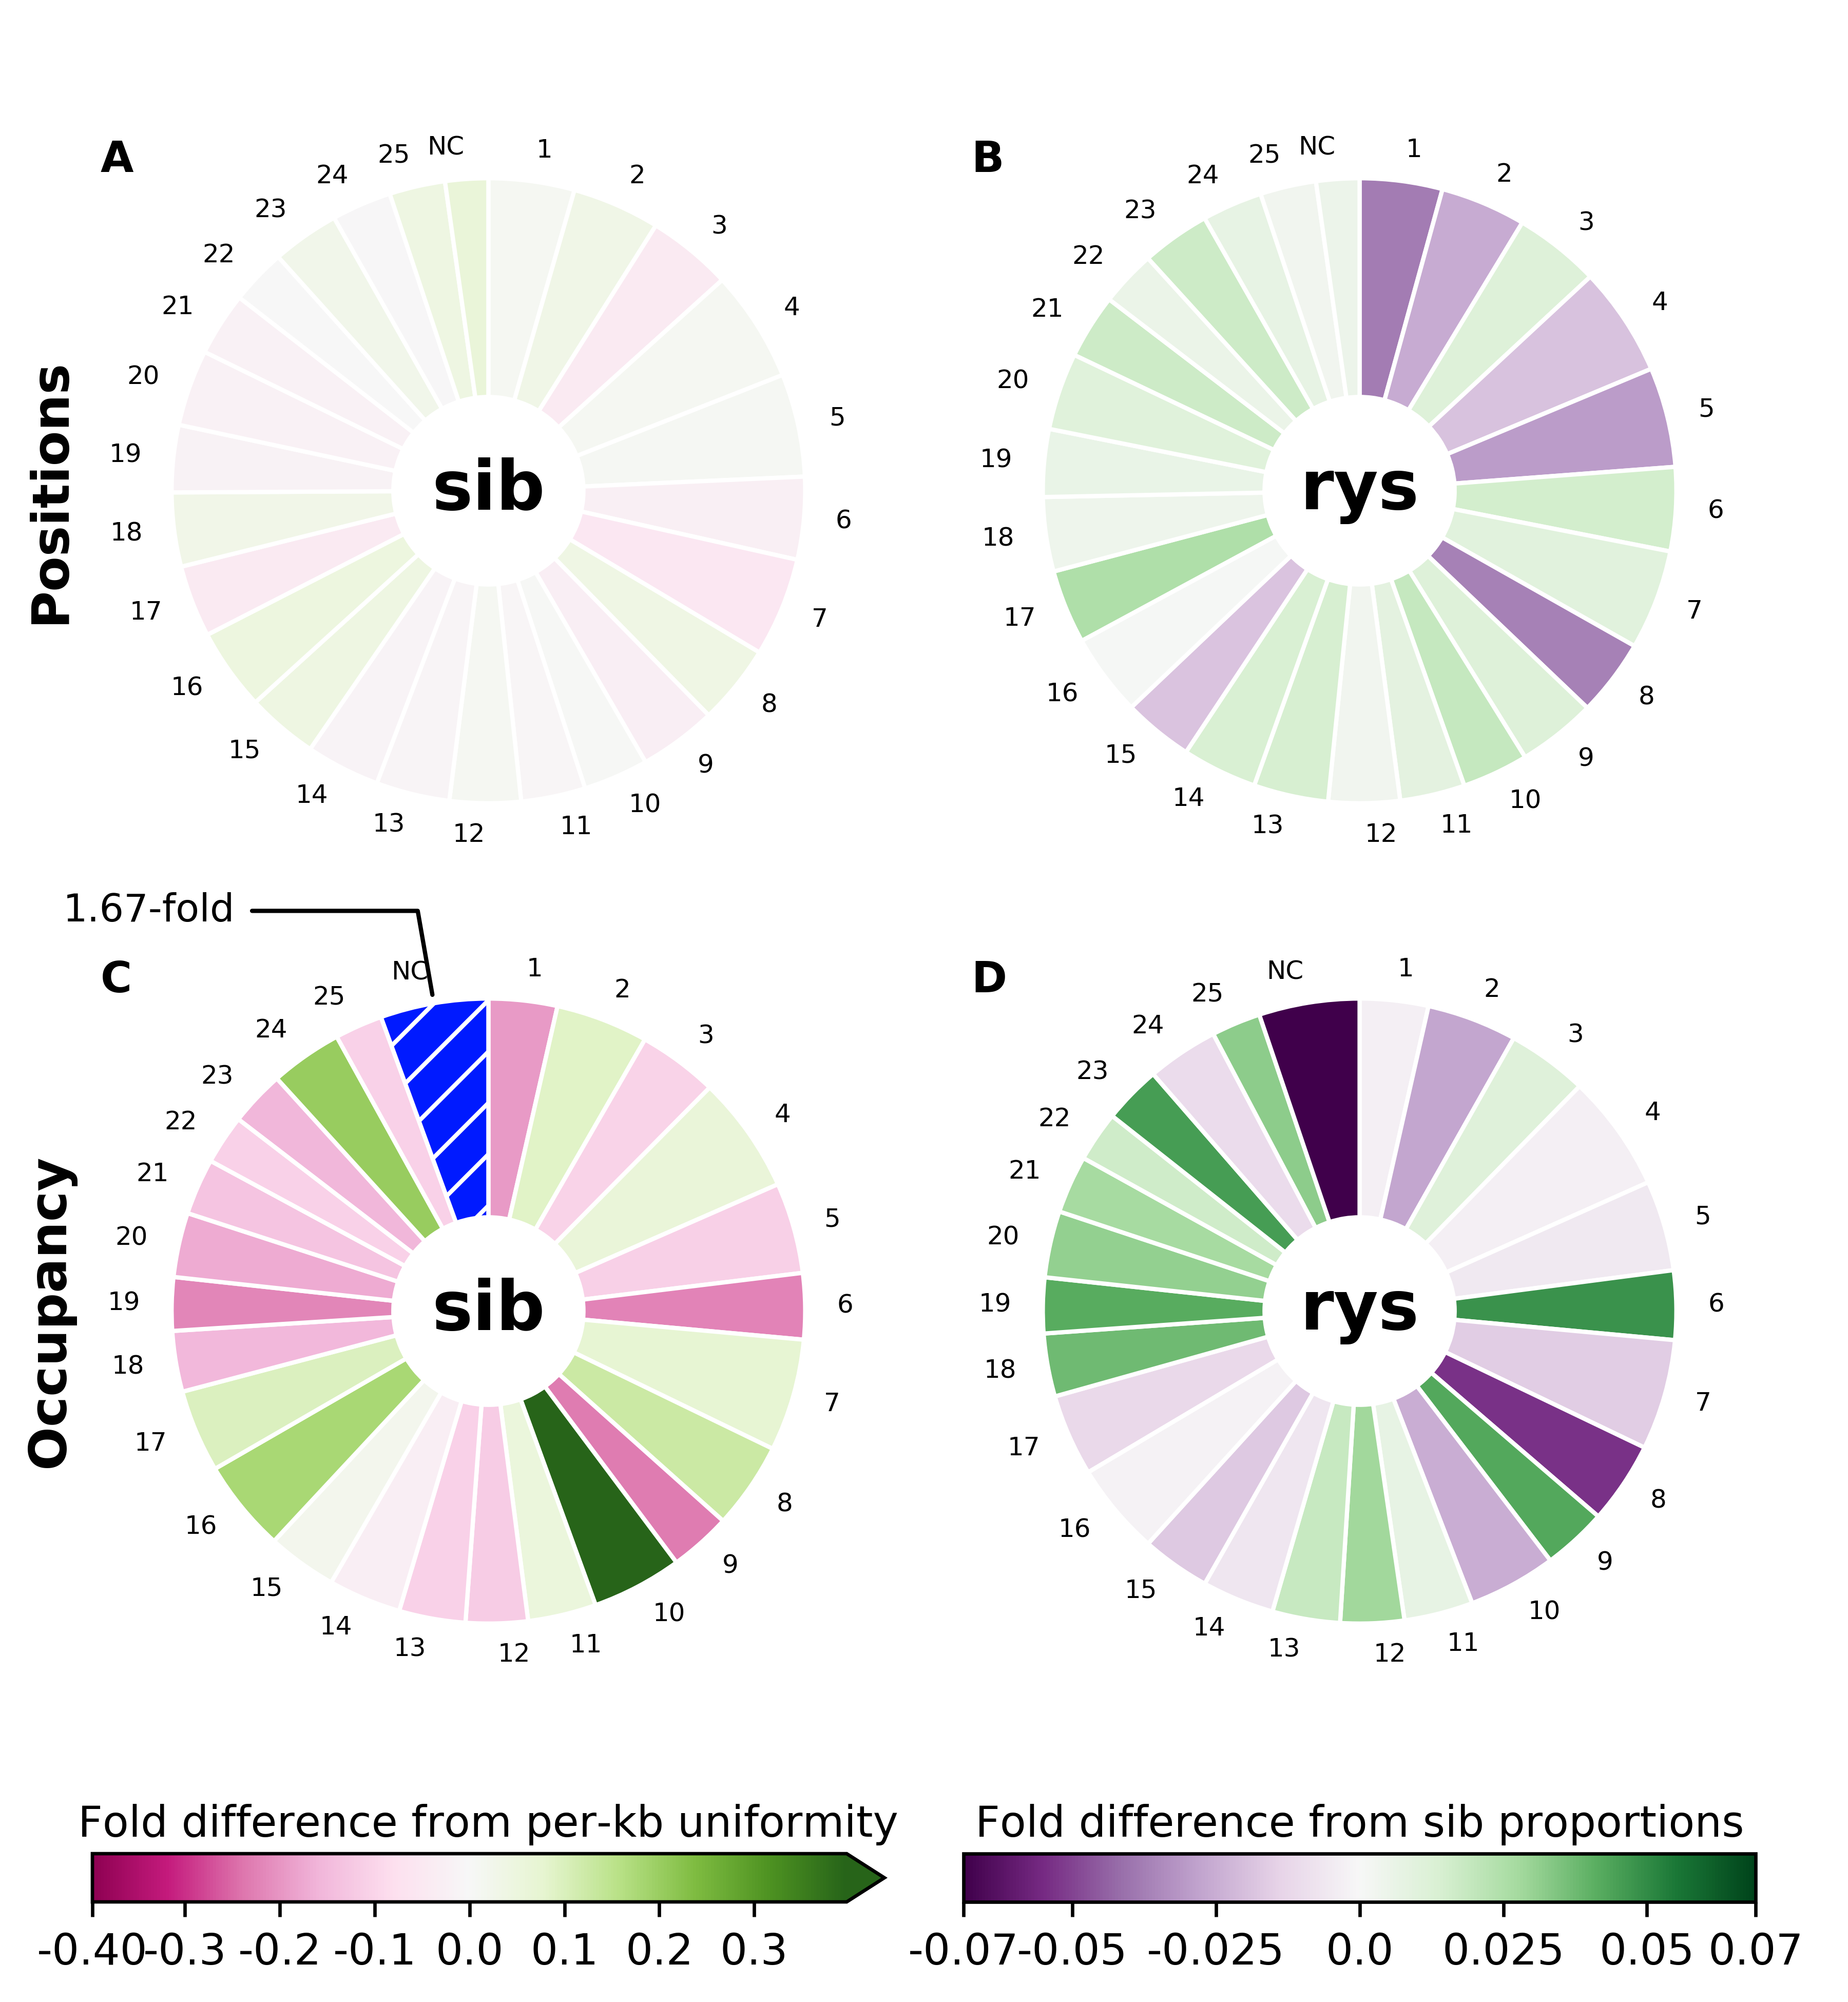
\includegraphics{rys/proportional_chromosome_occupancy.png}
\caption{{\bf rys chromosomes are differentially enriched and depleted of nucleosome position density and occupancy.}}
Pie charts of nucleosome position density and occupancy by chromosome. Width of pie slices in panels A and B indicates the fraction of the total number of positions occuring in the numbered chromosomes and nonchromosomal scaffolds (NC). In panel A, depicting the sib genome, slices are colored according to the extent of deviation from an assumption of even distribution of nucleosomes across the genome. In panel B, depicting the rys genome, slices are colored according to the extent of deviation from the sib distribution. The width of slices in slices B and D indicate the fraction of the total nucleosome occupancy signal detected. Slice coloration depicts deviations from nucleosome occupancy distributions analogous to position distributions in A and B. Blue and white diagonal bars in the NC slice of panel C denote an out-of-scale positive deviation from the assumption of even distribution, i.e., sib NC scaffolds have 1.67-fold more of the total nucleosome occupancy signal than is expected from their length alone.  
\label{nucgendist}
\end{figure}

By mapping the called nucleosome positions in rys to those in sibs, we observed that there is a subset of sib positions which are never found to be occupied in rys, and likewise a subset of rys positions which are unique to the mutants (Fig \ref{diffposdist}). Intriguingly, sib positions which are not observed in rys are compensated for quite evenly across the genome by new positions gained in the mutants, with a small excess of new rys positions on most chromosomes.


\begin{figure}[!h]
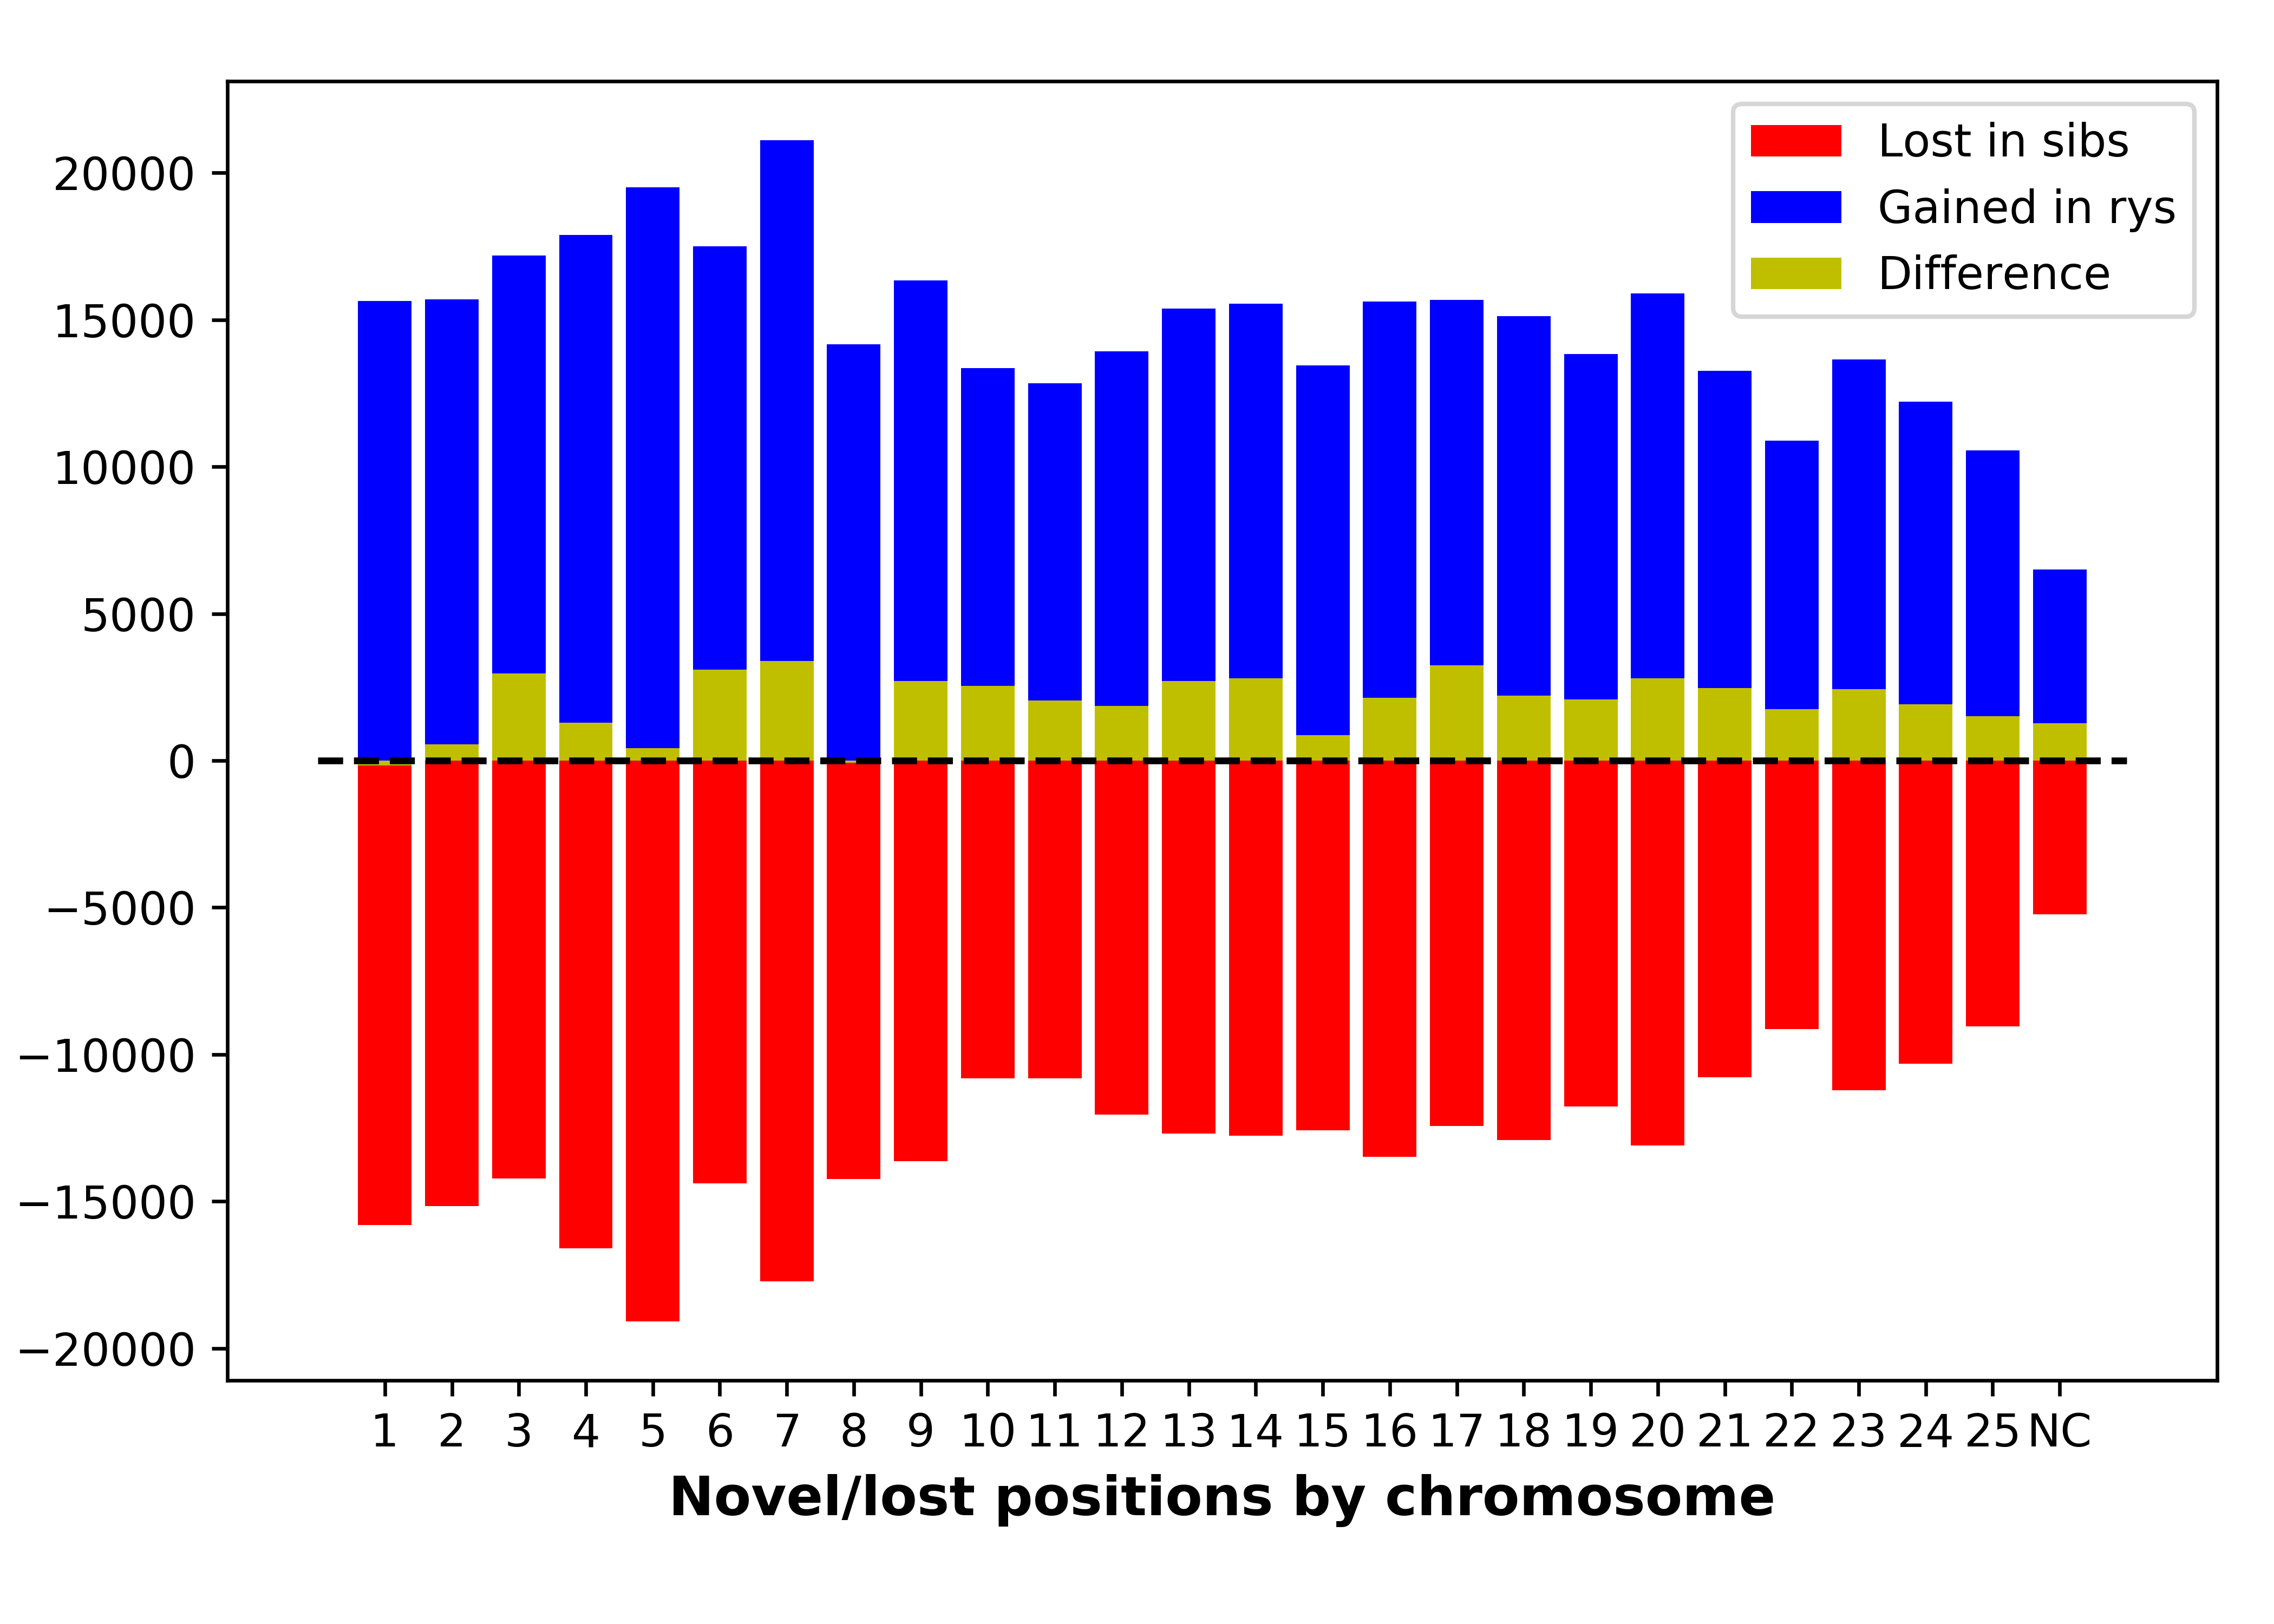
\includegraphics{rys/chr_unique_positions.png}
\caption{{\bf Novel nucleosome positions in rys occur in similar numbers to those lost from sibs.}}
Counts of positions found in sib but not rys (red bars, represented as negative numbers, as these are `lost' in rys) and those found in rys but not sib (blue bars, `gained'). The magnitude of the difference between the counts is represented with a yellow bar.
\label{diffposdist}
\end{figure}

This result suggested that a particular subpopulation of wild type nucleosomes are mislocalised in rys. If the pool of available histones in proliferating rys progenitors is substantially different from that of siblings, rys nucleosomes forming from this pool may have altered physico-chemical interactions with DNA, which could result in nucleosomes with unusual sequence preferences. If so, this would explain the disappearance of a subset of positions in rys and the appearance of a new, similarly sized subset of positions (the `differential set').

To formally address this hypothesis, we calculated the Bayesian evidence ratio for separate emission processes for sib and rys position sequences against a combined process for both sets of sequences. If the molecular process resulting in the differential set arises from altered nucleosome composition in proliferating rys cells, we expect these sequences to provide greater support for separate emission processes than for a single, combined process. On the other hand, if abberant DNA-nucleosome interaction is not causally relevant, and the reason for the apparently displaced nucleosomes is another macromolecular process, the evidence ratio should favour a combined process for the emission of the differential set- that is, there should be no difference between the unique sib and rys sequences that would justify the additional complexity of separate models.

To perform this calculation, we needed to construct background models of \textit{D. rerio}'s genomic "noise" from which repetitive sequence signals characteristic of nucleosome positions could be extracted. Following the suggestion of Down and Hubbard \cite{Down2005} that a principled approach to the selection of background models is to train and test a variety of them on relevant sequence, we used the Julia package BioBackgroundModels (BIORXIV CITE GOES HERE) to screen a panel of 1,2,4, and 6-state HMMS against  0th, 1st, and 2nd order encodings of samples from the zebrafish genome, partitioned grossly into exonic, periexonic, and intergenic sequences. We found that each of these partitions is best represented by 6-state HMMs trained on a 0th order genome encoding (i.e. the HMMs emit the 4 mononucleotides), as determined by model likelihood given an independent test sample, as displayed in Fig. \ref{BHMMlh}





In order to assess this, we performed micrococcal nuclease (MNase) digestion of genomic DNA (gDNA), and determined gross effects on polynucleosome organisation from gel analysis (Figure 5X). We subsequently performed MNase-Seq in order to map the specific positioning of nucleosomes on rys and sibling gDNA, and determined mapping analysis (Figure 5X). To confirm that chromatin organisation is indeed disrupted specifically in the CMZ, we acquired high-resolution transmission electron microscopy imagery of these cells in rys and sibling CMZs, observations from EM(Figure 5X).

\subsection{The rys CMZ does not contribute to the differentiated neural retina; the central retina of rys is disorganised}
Having characterised the effects of the rys npat mutation on the identity, nuclear organisation, and cell cycle of proliferating cells in the rys CMZ, we next addressed why rys mutant embryos are micropthalmic despite having a cycling pool of CMZ progenitors. To do so, we performed an EdU pulse-chase analysis of 3, 5, and 7 dpf rys and sibling embryos, pulsing these animals for 8 hours and subsequently chasing for 1 week before assaying for EdU reactivity. While rys siblings contribute new cohorts to all three layers of the neural retina normally at all time points (Figure 6A), the majority of rys mutants do not contribute to the differentiated neural retina at all at any timepoint (Figure 6B). [more specific quantitative analyses required] We also investigated whether mutant rys embryos have an associated central retinal phenotype by assaying for specific markers of differentiated retinal cell types (Table 1). We found that, while all examined markers are present in the correct layers, many cell types are disorganised or patchy relative to siblings (Figure 6C). more specific analyses of particular cell types? Eg zpr-1 photoreceptors

\subsection{The fate of rys CMZ cells is caspase-dependent apoptosis and subsequent phagocytosis by microglia}
Given that rys CMZ progenitors do not contribute to the neural retina, and that the population of rys CMZ cells is not expanded commensurately with their ongoing proliferation and failure to differentiate, we set out to determine what the fate of rys CMZ progeny might be. To investigate the possibility that rys CMZ cells may be dying in situ, we examined high-resolution TEM micrographs of rys CMZs for karyorrhectic nuclei and apoptotic bodies. We consistently observed these features in rys mutant but not sibling CMZs (Figure 8A). Caspase-3 immunoreactivity of rys CMZs was also assayed; we found significantly more caspase-positive cells in rys mutant relative to sibling CMZs (n=??; p<??)(Figure 8B). Finally using an antibody directed to 4C4, an epitope associated with zebrafish microglia, in combination with TUNEL staining, we observed TUNEL-labelled bodies internalised in 4C4-positive microglia in rys mutants significantly more frequently than in rys siblings (n=??; p<??)(Figure 8C).

\section{Discussion}
The zebrafish rys mutant model provides a heretofore unique opportunity to study the role of an NPAT homologue in a complete, developing tissue. This has previously proven difficult using mouse Npat, proviral inactivation of which resulted in early embryonic arrest, prior to tissue formation (Di Fruscio1997). The survival and development of rys mutant embryos beyond this stage may reflect the presence of wild-type npat transcript contributed maternally \cite{Harvey2013}; rys mutants nevertheless do not survive beyond metapmorhosis (\textasciitilde{}21dpf), so npat seems to be similarly obligatory for normal development in zebrafish, if over a longer timeframe.
As teleost fish are known to have undergone whole-genome duplication subsequent to their radiation from vertebrates, it is possible that zebrafish may have multiple npat paralogues. We have excluded this possibility due to our failure to identify any significantly similar CDS sequences in the Zv9 zebrafish genome using BLAST. The zebrafish npat gene does have a substantially different genomic context from human NPAT, however: it is not associated with the eponymous ATM locus (which has been duplicated, and is present in this duplicate form elsewhere on chromosome 15). ATM’s 5’ position is, in zebrafish, occupied by hif1al, with the intergenic region lacking canonical E2F promoter sites. Of the 80 vertebrate genomes currently available from Ensembl, this organisation is shared only with the cave fish (A. mexicanus), with the human-like ATM-NPAT association preserved in all other species. This apparently evolutionarily novel genomic organisation for npat may be responsible for some of the differences in npat function we report here relative to its homologues.
The rys mutation in zebrafish npat is associated with gross abnormalities in CMZ nuclear organisation and altered expression of progenitor markers. These changes were observed with a concomitantly shortened S-phase, a phenomenon which has not previously been reported in any NPAT mutant, knockout, or knockdown context. A shortened S-phase is nonetheless a viable alternative interpretation of some prior work; Gao et al. \cite{Gao2003}, for instance, reported a decline in the number of cells in S-phase in a population of synchronised U2OS cells treated with siRNAs directed against NPAT, coupled with an increase in the number of cells in G2/M. This was interpreted as a decreased propensity of NPAT-knockdown cells to proceed through the G1/S barrier, but could also be explained by a shortened S-phase resulting in fewer cells in S and faster progression to G2/M phase. Unfortunately, no experiments have been conducted with the robust cumulative thymidine analogue labelling paradigm we use here, so it remains unclear whether the observed truncated S phase is unique to rys or if it might be present in other contexts as well.
We subsequently identified alterations in histone mRNA transcription and 3’ end processing as candidate mechanisms by which the rys phenotype might be produced. In both 6 and 8 dpf rys larvae as well as npat-morpholino treated 1dpf embryos, we observe increased abundances of histone and, specifically, polyadenylated histone transcripts, although the composition of affected histone families differs between these contexts. The specific mechanism by which these effects are produced in rys remains unclear, and the increases in histone transcript abundance observed in both mutant and morpholino-treated animals is at odds with observations that NPAT knockouts display decreases in histone transcription \cite{Ye2003} and that the destruction of CDK phosphorylation sites on NPAT protein, which has putatively occurred in the rys npat protein, or treatment with a CDK inhibitor, result in similar declines in histone transcript abundance \cite{Ma2000,Mitra2009}. This may imply the role of zebrafish npat in regulating histone transcription is be structurally different from what has been described for human NPAT. We are unable to determine from these data whether the overall increases histone transcript abundance are a consequence of increased histone transcription or of the greater stability of improperly polyadenylated histone transcript, however. The increased abundance of polyadenylated transcript in rys mutants and npat morpholino-treated embryos is consistent with the observed role of NPAT in recruiting CDK9 to replication-dependent histone gene clusters, known to be important in generating the normal stem-loop structure at the 3’ end of these transcripts \cite{Pirngruber2009}, suggesting that this role is conserved in zebrafish. It is also possible that particular histone genes give rise to polyadenylated transcripts in zebrafish, as observed in a variety of cell lines \cite{Kari2013}; increased transcription of these particular genes might also account for the observed increase in polyadenylated histone transcript abundance. We speculate that the increased abundance of histone transcript in rys allows for more rapid, if dysfunctional, chromatin packaging, and consequently the shorter S-phase observed in the CMZ of these animals.
Interestingly, although increased abundance of polyadenylated histone transcript has been associated with both cell cycle arrest and differentiation \cite{Kari2013}, we found that in the rys mutant CMZ, this was associated with altered cell cycle parameters, failure to differentiate, and ultimately, cell death by apoptosis. This suggests that the presence of polyadenylated histone transcripts are not directly related to particular cell cycle states or differentiated fates, but rather that a particular regime of coordination and control of the expression of polyadenylated and replication-dependent, stem-looped histone transcripts is required to achieve appropriate transitions between these states. In the case of rys, this seems to be related to the effect of altered histone expression on chromatin structure; we observed in the rys mutant CMZ altered nuclear morphology, chromatin ultrastructural features, and nucleosome positioning. As the spatiotemporal dynamics of chromatin architecture are known to be critically involved in both replication timing \cite{Gilbert2010} and cell identity and fate \cite{Serrano2013}, the significant alterations we observe in rys mutant chromatin architecture, accompanied by our observations of altered cell identity marker expression [proteomics analyisis references] provide a plausible molecular mechanism by which mutated npat protein can produce the observed components of the rys mutant CMZ phenotype via altered histone expression. Further experimentation is required to determine how specific changes in chromosome organisation (e.g. alterations in 3-dimensional chromatin organisation of gene expression, number of replication foci, etc.) produce specific features of the rys phenotype. 
The rys npat mutant has also provided an opportunity to elucidate some heretofore obscure features of the zebrafish retina. We found that the failure of the rys mutant CMZ to contribute to the differentiated neural retina was associated with a phenotype of progressive disorganisation in the central retina, which may suggest either that CMZ contributions are required to maintain the normal ordering of the retina over time, or that npat has a previously unrecognised role in patterning and maintaining the viability of differentiated retinal neurons. Furthermore, we identified microglia as the cells responsible for the phagocytosis of dying cells at the retinal periphery in rys mutants, an activity which has not previously been ascribed to these neural immune cells. This behaviour on the part of microglia may be necessary for the homeostasis of the CMZ proliferative niche, and may in part explain the ability of the rys mutant CMZ to remain relatively intact for an extended period of time in spite of the failure of its progeny to differentiate and their eventual apoptotic fate. 
